Using Matlab, the following discrete-time pulse sequences are to be visualized in the time range of $n \in [-20,20]$

\begin{flalign*}
	s_1[n]&=\delta[n]\quad\textrm{(Dirac delta function)} \\
	s_2[n]&=\sigma[n]\quad\textrm{(snap-action function(Sprungfunktion))} \\
	s_3[n]&=\begin{cases}
		0,\: \textrm{für} \quad n \leq 0 \\
		n,\: \textrm{für} \quad n > 0
	\end{cases} \\
	s_4[n]&=\begin{cases}
		-2,&\: \textrm{für} \quad n \leq -2 \\
		n,&\: \textrm{für} \quad -2 < n < 2 \\
		2,&\: \textrm{für} \quad n \geq 2
	\end{cases}
\end{flalign*}

\lstinputlisting[language=Matlab]{./assets/Lab1_419.m}
{
	\setlength{\fboxsep}{0pt}%  
	\colorbox{backcolor}{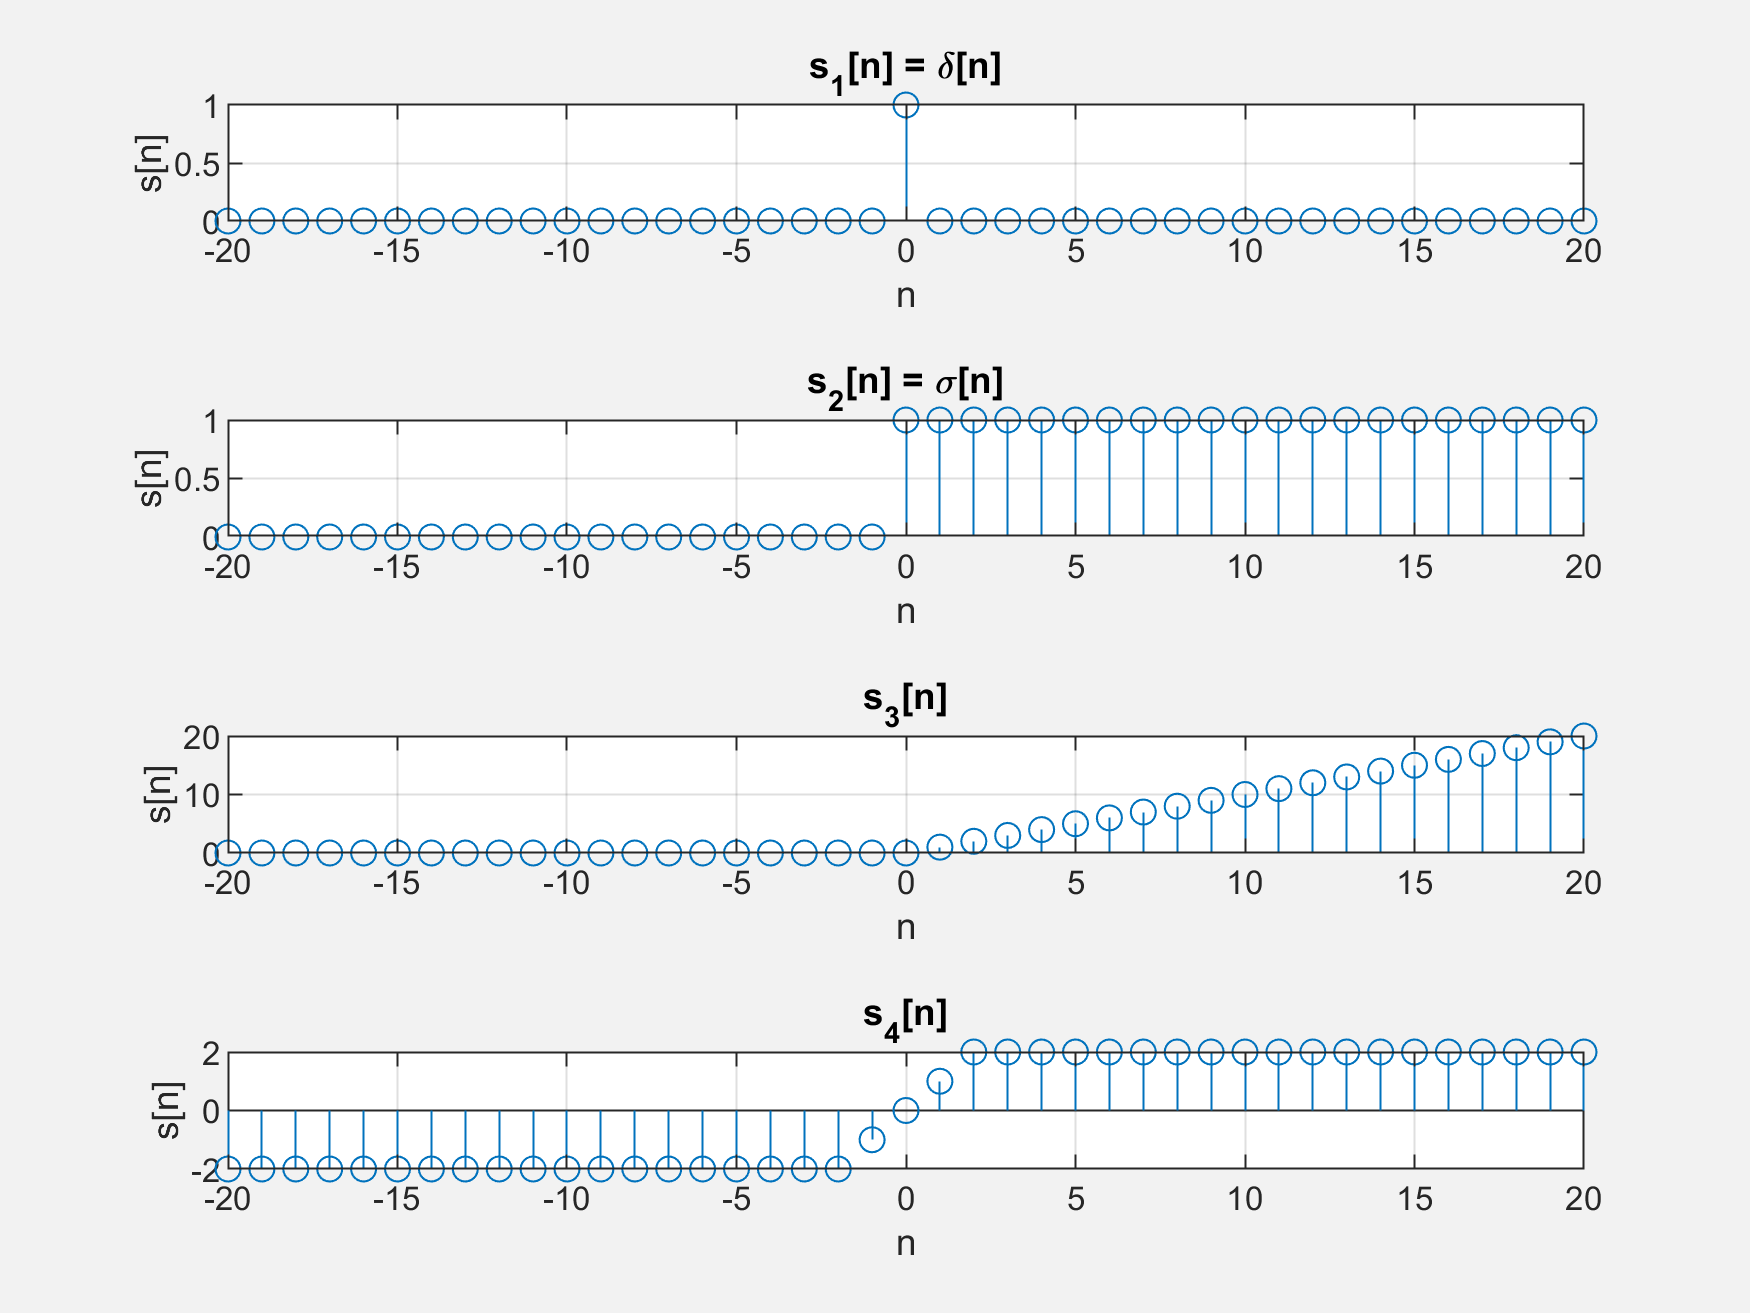
\includegraphics[width=\linewidth, keepaspectratio]{./assets/419.png}}
}